\documentclass{article}

\usepackage{fullpage}
\usepackage[utf8]{inputenc}
\usepackage{listings}
\usepackage{caption}
\usepackage{subcaption}
\usepackage[svgnames]{xcolor}
\usepackage{amssymb}
\usepackage{amsmath}
\usepackage{fancyhdr}
\usepackage{lastpage}
\usepackage{parskip}
\usepackage{abstract}
\usepackage{gensymb}
\usepackage{url}
\usepackage{float}
\usepackage{enumitem}
\usepackage{amstext}
\usepackage{fancybox}
\usepackage{amsmath}
\usepackage{graphicx}
%\usepackage{subfigure}
\usepackage[bottom]{footmisc}
\usepackage{hyperref}
\usepackage{tikz}
\usepackage{makecell}
\usepackage{tabulary}
\usepackage{pdfpages}
\usepackage{verbatim}
\usepackage{tikz}
\usetikzlibrary{positioning}
\usetikzlibrary{arrows}
\pagenumbering{gobble}

\setcounter{secnumdepth}{3} % only chapter and sections will be numbered
\setcounter{tocdepth}{3}    % entries down to \subsubsections in the TOC


\begin{document}

\section*{1 - Compiler optimization}
\begin{enumerate}
	\item Loop-optimization: Move loop-invariant variables outside the loop.
	\item Dead code removal.
	\item Subexpression elimination: (x + y) / 3.0 - (x + y)
	\item Replacing instructions with more efficient ones. For instance, x = x * 2 is likely faster performed by bitshifting
\end{enumerate}

Primarily optimizing either for (run) time or for space.



\section*{3 - Explain components in compilation toolchain}
\begin{enumerate}
	\item Source file(s) are handled by the preprocessor, which turn them into \textbf{translation units}:
	\begin{itemize}
		\item The preprocesser recursively includes files marked by \#include
		\item The preprocesser expands macros such as \#if, \#define, \#ifdef
	\end{itemize}
	Translation units consists of declarations and definitions.
	\item Each translation unit is then \emph{compiled} into object files
	\item Object files can then, together with (static) libraries, be linked into executables.
\end{enumerate}

\textbf{Remember} that there are both \emph{static} and \emph{dynamic} libraries. Static are linked into the executable, whereas dynamic can be changed (updated) with time (dynamic linked).


\section*{4 - Memory leaks in systems with dynamic memory management}
\subsection*{How they can occur}
\begin{itemize}
	\item In the C standard library, one can call \texttt{malloc()} to get a pointer to the memory of the requested size.
 If one deletes the pointers to the allocated data, without freeing the memory block before, this is a memory leak. 
 
 	\item Memory fragmentation
\end{itemize}


\subsection*{2 strategies to prevent them}
\begin{itemize}
	\item Garbage collection. Detect data objects that cannot be used by the program in the future, and free the resources occupied by these.
	\item TODO:
\end{itemize}


\section*{5 - Explain the diff. between communicating with an I/O device using memory mapped I/O or I/O-instructions}
TODO: !!! 

\section*{6 - Explain processor, register, program counter, cache, I/O device, instruction set architecture}

\begin{center}
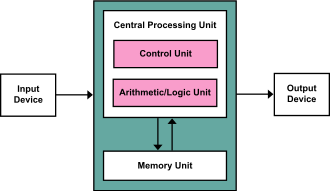
\includegraphics[width=8.0cm]{images/330px-Von_Neumann_Architecture.png}

Von Neumann Architecture
\end{center}


\subsection*{Processor}
There are different kinds of processors, the most widely used are
\begin{itemize}
	\item General purpose central processing units (CPUs, used in PCs)
	\item ASIC (application-specific integrated circuit)
	\item GPU (graphics processing units)
\end{itemize}

Operates in \textbf{cycles}:
\begin{itemize}
	\item Fetch instruction (using the PC/IP)
	\item Decode instruction (there are different \emph{addressing modes})
	\item Execute - Control Unit and ALU (Arithmetic/Logic Unit)
\end{itemize}

\textbf{Word size} - Modern PCs use a word-size of 64 bits. Embedded systems using microcontrollers often have a smaller word size

\subsection*{Register}
Lulz

\subsection*{Program counter / instruction pointer (PC/IP)}
So... yeah.

\subsection*{Cache}
TODO: cache coherence - when there are multiple caches for multiple processors. These must be kept consistent.

\subsection*{I/O device}

\subsection*{Instruction set architecture (ISA)}
Well-defined software/hardware interface.

\begin{itemize}
	\item Functional definition - Operations and storage locations supported by hardware. With Intel's Ivy Bridge chip-architecture came the operation RdRand for instance, which is an operation that returns a hardware-generated random number.
	\item Documentation of how to use the instructions (see ABI below?).
\end{itemize}

(TODO: application binary interface (ABI). I believe this is contained within ISA. This defines the calling conventions for the architecture - for instance how system calls are carried out)

\section*{10 - draw a figure showing how the memory hierarchy of a modern computer with the processor(s), cache levels, memory and storage}

\begin{center}
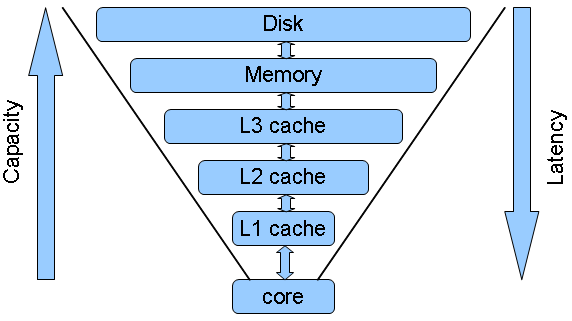
\includegraphics[width=5.0cm]{images/cpu_cache_structure.png}
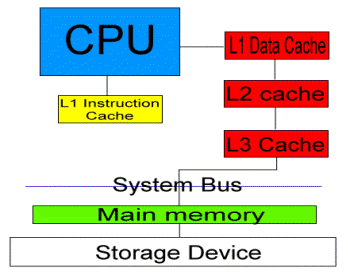
\includegraphics[width=5.0cm]{images/CPU-Cache-System.png}



Simplified overviews of CPU, registers, caches and memory
\end{center}

\emph{L1} is often local for each CPU, whereas \emph{L2} and/or \emph{L3} are/is often shared between multiple CPUs.

\emph{Extremely} important: When you draw the storage, remember to draw it as a cylinder\footnote{due to historical reasons}!


\section*{C - interrupts!}
TODO: fuck fuck fuck


\section*{C - storage classes (week 2)}
TODO: auto, extern, static and register!


\section*{Memory layout (week3)}
TODO: (memory areas) How are they laid out? In what order Where in memory?



\section*{20}
Given reference literature, you can write down in text and in your own words definitions or explanations of the following concepts:

\begin{description}
\item[Process Address space]
  The actual address space taken allocated to a process in a virtual address space.

\item[Interprocess communication]
  Can be done in numerous ways: files, message queues, semaphore, message passing, shared memory, pipes (IO), and more.

\item[System call]
  A program's request to the operating system to do an OS tasks

\item[Daemon]
  A process running in the background (``invisible''), can be a watchdog-like program, auto-updater, anti-virus, etc.

\item[Thread]
  Smallest ``unit'' known by the scheduler. Owned by a process. Threads of the same process share memory.

\item[Critical section]
  A piece of code that needs mutual exclusion. A critical \texttt{region} consists of multiple of these.

\item[Mutual exclusion]
  Ya kno dis

\item[Semaphore]
  P = request/take coconut, V = put coconut

\item[Mutex]
  Binary semaphore, a simple lock/unlock mechanism

\item[Monitor]
  A construct (class, object, whatever) with mutual exclusion of methods

\item[Condition variable]
  In a Java monitor it's the \texttt{wait} and \texttt{notify} and \texttt{notifyAll}. It's the mechanism by which a monitor can wait for a condition to be true without blocking the monitor.

\item[Message passing]
  Communication between objects in the same process or between different processes by use of so-called messages. Can be asynchronous or synchronous. Invoking a method on an object in Java is an example of message passing, and sending a signal from one process to another in unix with \texttt{kill} is another.

\item[Kernel mode]
  One of the two modes of operation of the CPU. In kernel mode all code executed is \textit{trusted} so it can access all memory, signal all processes, execute all instructions, etc.

\item[User mode]
  One of the two modes of operation of the CPU. In user mode code is not assumed to be \textit{trusted} so it is restricted to a certain memory space and possibly a limited subset of CPU instructions.

\item[Pre-emtiveness]
  A preemption happens when a process is suspended \textit{during} its execution, resulting in a \textit{context switch}, usually done by the scheduler. The intent is that the process will be resumed later.

\item[Race condition]
  Happens when two processes attempts to access/mutate a shared resources at the same time, such that unexpected behavior or corruption can occur.

\item[Scheduling algorithm]
  Algorithm that chooses which processes (or threads) to execute.

\item[System time]
  The computer's time ``counter''

\item[Device driver]
  Program that controls a hardware device and provides an interface to it (usually through the bus)

\end{description}


























\end{document}